%%%%%%%%%%%%%%%%%%%%%%%%%%%%%%%%%%%%%%%%%%%%%%%%%%%%%%%%%
\begin{frame}[fragile]{사원수}

\begin{itemize}
\item 사원수(quaternion)는 스칼라(scalar) 값과 3차원 벡터를 묶어 구성한 복소수(complex number)
\item 3차원 벡터 $\mathbf v = (a, b, c)$를 각각의 축 방향 단위 벡터인 기저 $\mathbf i, \mathbf  j, \mathbf k$로 표현하면 $a{\mathbf i} + b {\mathbf j} + c {\mathbf k}$
\item 사원수는 여기에 스칼라 값 $d$가 추가된 $d + a{\mathbf i} + b {\mathbf j} + c {\mathbf k}$
\item 기저를 제외하고 표현하면 $(d, (a, b, c))$와 같이 표현 
\item 벡터 기호로 표현하면 $(d, \mathbf v)$
\item 스칼라 값은 기저가 실수의 단위 값인 1이라고 이해하면 사원수는 $1, \mathbf i, \mathbf  j, \mathbf k$를 기저로 하는 벡터
\item 로보틱스와 컴퓨터 그래픽스 분야에서 회전을 다루는 데에 빈번히 이용
\end{itemize}

\end{frame}
%%%%%%%%%%%%%%%%%%%%%%%%%%%%%%%%%%%%%%%%%%%%%%%%%%%%%%%%%

%%%%%%%%%%%%%%%%%%%%%%%%%%%%%%%%%%%%%%%%%%%%%%%%%%%%%%%%%
\begin{frame}[fragile]{사원수의 연산 - 덧셈과 뺄셈}

\begin{itemize}
\item 사원수 덧셈: 성분별로 더하면 된다.
\item 두 개의 사원수 $\hat{p}$와 $\hat{q}$가 각각 $(s_p, \mathbf v_p)$와 $(s_q, \mathbf v_q)$일 때, 덧셈은
	\begin{itemize}
	\item $\hat{p} + \hat{q} = (s_p + s_q , \mathbf v_p + \mathbf v_q )$
	\item $\hat{p} = (a_p, b_p, c_p, d_p)$와 $\hat{q} = (a_q, b_q, c_q, d_q)$
		\begin{itemize}
		\item $\hat{p} + \hat{q} = (a_p + a_q, b_p + b_q , c_p + c_q , d_p + d_q)$
		\end{itemize}
	\end{itemize}
\end{itemize}

\begin{itemize}
\item 뺄셈
	\begin{itemize}
	\item $\hat{p} - \hat{q} = (a_p - a_q, b_p - b_q , c_p - c_q , d_p - d_q)$
	\item 스칼라와 벡터로 나누어 표현하면 다음과 같다.
		\begin{itemize}
		\item $\hat{p} = (s_p, \mathbf v_p),~~~ \hat{q} = (s_q, \mathbf v_q)$
		\item $\hat{p} + \hat{q} = (s_p - s_q , \mathbf v_p - \mathbf v_q )$
		\end{itemize}
	\end{itemize}
\end{itemize}

\end{frame}
%%%%%%%%%%%%%%%%%%%%%%%%%%%%%%%%%%%%%%%%%%%%%%%%%%%%%%%%%



%%%%%%%%%%%%%%%%%%%%%%%%%%%%%%%%%%%%%%%%%%%%%%%%%%%%%%%%%
\begin{frame}[fragile]{사원수의 연산 - 스칼라 곱셈}

사원수와 어떤 스칼라 $\lambda$를 곱하는 것은 모든 성분에 이 스칼라 값을 곱하는 것이다.

$$\lambda \hat{p} = (\lambda s_p , \lambda \mathbf v_p) = (\lambda a_p, \lambda b_p, \lambda c_p, \lambda d_p)$$




\end{frame}
%%%%%%%%%%%%%%%%%%%%%%%%%%%%%%%%%%%%%%%%%%%%%%%%%%%%%%%%%

%%%%%%%%%%%%%%%%%%%%%%%%%%%%%%%%%%%%%%%%%%%%%%%%%%%%%%%%%
\begin{frame}[fragile]{사원수의 연산 - 사원수 곱셈 1/4}

\begin{itemize}
\item 두 사원수 $\hat{p}$와 $\hat{q}$를 곱하려면 어떻게 해야 할까?
\item 사원수는 서로 다른 허수 $\mathbf i, \mathbf j, \mathbf k$를 가진 벡터와 스칼라의 합인 복소수
\item 허수들 사이의 곱
	\begin{itemize}
	\item $\mathbf i^2 = \mathbf j^2 = \mathbf k^2 = -1$
	\item $\mathbf {ij} = \mathbf k$, $\mathbf {jk} = \mathbf i$, $\mathbf {ki} = \mathbf j$
	\item $\mathbf {ji} = -\mathbf k$, $\mathbf {kj} = -\mathbf i$, $\mathbf {ik} = -\mathbf j$
	\end{itemize}
\item $\hat{p} \hat{q}$는 다음과 같이 표현 가능
	\begin{itemize}
	\item $\hat{p}  =  d_p + a_p{\mathbf i} + b_p{\mathbf j} + c_p{\mathbf k}$
	\item $\hat{q}  =  d_q + a_q{\mathbf i} + b_q{\mathbf j} + c_q{\mathbf k}$
	\end{itemize}
\end{itemize}

\begin{eqnarray}
\hat{p}\hat{q} = &
d_p d_q + d_p + d_p a_q{\mathbf i} + d_p b_q{\mathbf j} + d_p c_q{\mathbf k} + \nonumber \\
& a_p {\mathbf i} d_q + a_p {\mathbf i}  a_q{\mathbf i} + a_p {\mathbf i} b_q{\mathbf j} + a_p {\mathbf i}  c_q{\mathbf k} + \nonumber \\
& b_p {\mathbf j} d_q + b_p {\mathbf j} a_q{\mathbf i} + b_p {\mathbf j} b_q{\mathbf j} + b_p {\mathbf j} c_q{\mathbf k} + \nonumber \\
& c_p {\mathbf k} d_q + c_p {\mathbf k} a_q{\mathbf i} + c_p {\mathbf k} b_q{\mathbf j} + c_p {\mathbf k} c_q{\mathbf k}  \nonumber
\end{eqnarray}

\end{frame}
%%%%%%%%%%%%%%%%%%%%%%%%%%%%%%%%%%%%%%%%%%%%%%%%%%%%%%%%%

%%%%%%%%%%%%%%%%%%%%%%%%%%%%%%%%%%%%%%%%%%%%%%%%%%%%%%%%%
\begin{frame}[fragile]{사원수의 연산 - 사원수 곱셈 2/4}

정리하면 다음과 같다. 

\begin{eqnarray}
\hat{p}\hat{q} = &
d_p d_q + d_p a_q{\mathbf i} + d_p b_q{\mathbf j} + d_p c_q{\mathbf k} + \\ \nonumber
& a_p d_q{\mathbf i}  + a_p a_q {\mathbf i}^2 + a_p b_q{\mathbf i} {\mathbf j} + a_p c_q {\mathbf i}  {\mathbf k} + \\ \nonumber
& b_p d_q {\mathbf j} + b_p a_q {\mathbf j} {\mathbf i} + b_p b_q{\mathbf j}^2 + b_p c_q {\mathbf j} {\mathbf k} + \\ \nonumber
& c_p d_q{\mathbf k}  + c_p a_q{\mathbf k} {\mathbf i} + c_p b_q{\mathbf k} {\mathbf j} + c_p c_q {\mathbf k}^2
\end{eqnarray}

허수의 곱이 나타나는 부분을 정리하면,

\begin{eqnarray}
\hat{p}\hat{q} = &
d_p d_q + d_p a_q{\mathbf i} + d_p b_q{\mathbf j} + d_p c_q{\mathbf k} + \\ \nonumber
& a_p d_q{\mathbf i}  - a_p a_q + a_p b_q{\mathbf k} - a_p c_q {\mathbf j} + \\ \nonumber
& b_p d_q {\mathbf j} - b_p a_q {\mathbf k} - b_p b_q + b_p c_q {\mathbf i} + \\ \nonumber
& c_p d_q {\mathbf k}  + c_p a_q{\mathbf j} - c_p b_q{\mathbf i} - c_p c_q 
\end{eqnarray}


\end{frame}
%%%%%%%%%%%%%%%%%%%%%%%%%%%%%%%%%%%%%%%%%%%%%%%%%%%%%%%%%


%%%%%%%%%%%%%%%%%%%%%%%%%%%%%%%%%%%%%%%%%%%%%%%%%%%%%%%%%
\begin{frame}[fragile]{사원수의 연산 - 사원수 곱셈 3/4}

허수별로 정리하면 다음과 같다.

\begin{eqnarray}\nonumber
\hat{p}\hat{q} = & d_p d_q  - a_p a_q - b_p b_q - c_p c_q  \\ \nonumber
&+ d_p a_q{\mathbf i} + a_p d_q{\mathbf i} + (b_p c_q - c_p b_q ) {\mathbf i}  \\ \nonumber
&+ d_p b_q{\mathbf j} + b_p d_q {\mathbf j} + (c_p a_q - a_p c_q) {\mathbf j} \\ \nonumber
&+ d_p c_q{\mathbf k} + c_p d_q {\mathbf k} + (a_p b_q - b_p a_q) {\mathbf k} \nonumber
\end{eqnarray}


계산의 의미는 다음과 같다.

\begin{eqnarray} \nonumber
\hat{p}\hat{q} = & d_p d_q  - (a_p a_q + b_p b_q + c_p c_q)  \\ \nonumber
&+ d_p ( a_q{\mathbf i} + b_q {\mathbf j} + c_q {\mathbf k}) \\ \nonumber
&+ d_q ( a_p{\mathbf i} + b_p {\mathbf j} + c_p {\mathbf k}) \\ \nonumber
&+ (b_p c_q - c_p b_q ) {\mathbf i}  + (c_p a_q - a_p c_q) {\mathbf j} + (a_p b_q - b_p a_q) {\mathbf k} \nonumber
\end{eqnarray}


\end{frame}
%%%%%%%%%%%%%%%%%%%%%%%%%%%%%%%%%%%%%%%%%%%%%%%%%%%%%%%%%

%%%%%%%%%%%%%%%%%%%%%%%%%%%%%%%%%%%%%%%%%%%%%%%%%%%%%%%%%
\begin{frame}[fragile]{사원수의 연산 - 사원수 곱셈 4/4}

{\small
벡터의 내적과 외적을 이용하여 설명하면,

\begin{eqnarray}\nonumber
\hat{p}\hat{q} = & d_p d_q  - (\mathbf v_p \cdot \mathbf v_q)  \\ \nonumber
&+ d_p \mathbf v_q + d_q \mathbf v_p + \mathbf v_p \times \mathbf v_q \nonumber
\end{eqnarray}


사원수를 스칼라 값과 벡터 표현인 $(d, \mathbf v)$로 표현하면,
\begin{eqnarray}\nonumber
\hat{p}\hat{q} & = & (d_p, \mathbf v_p) (d_q , \mathbf v_q) \\ \nonumber
& =  & ( d_p d_q  - \mathbf v_p \cdot \mathbf v_q , ~~~ d_p \mathbf v_q + d_q \mathbf v_p + \mathbf v_p \times \mathbf v_q ) \nonumber
\end{eqnarray}


\begin{itemize}
\item 스칼라: 두 사원수가 가진 스칼라 값의 곱에서 두 사원수가 가진 벡터 내적을 뺀 것
\item 벡터: 각 사원수가 가진 스칼라 값을 상대편의 벡터 부분에 곱한 결과 두 개를 더하고, 두 사원수가 가진 벡터를 서로 외적하여 얻는 벡터를 추가로 더하여 얻음
\end{itemize}
}

\end{frame}
%%%%%%%%%%%%%%%%%%%%%%%%%%%%%%%%%%%%%%%%%%%%%%%%%%%%%%%%%

%%%%%%%%%%%%%%%%%%%%%%%%%%%%%%%%%%%%%%%%%%%%%%%%%%%%%%%%%
\begin{frame}[fragile]{사원수의 연산 규칙}

$$\hat{p} + \hat{q} = \hat{q} + \hat{p}$$
$$(\hat{p} + \hat{q}) + \hat{r} = \hat{p} + (\hat{q} + \hat{r} )$$
$$\lambda \hat p = \hat p \lambda$$
$$- \lambda \hat p = \lambda ( - \hat p)$$
$$\hat p \hat q \neq \hat q \hat p$$

\end{frame}
%%%%%%%%%%%%%%%%%%%%%%%%%%%%%%%%%%%%%%%%%%%%%%%%%%%%%%%%%


%%%%%%%%%%%%%%%%%%%%%%%%%%%%%%%%%%%%%%%%%%%%%%%%%%%%%%%%%
\begin{frame}[fragile]{켤레 사원수 1/2}

\begin{itemize}
\item 켤레 사원수(공액 사원수, conjugate)
	\begin{itemize}
	\item 어떤 사원수 $\hat p = (d_p, \mathbf v_p)$의 켤레 사원수를 $\hat p^*$라고 표현
	\item 이 켤레 이 사원수는 $(d_p, - \mathbf v_p)$의 값을 가짐
	\end{itemize}
\end{itemize}

$$\hat p = (d_p ,  \mathbf v_p) \Rightarrow \hat p^* = (d_p , -\mathbf v_p)$$

\begin{itemize}
\item 사원수의 크기는 벡터의 크기와 같은 방식으로 구한다.
\end{itemize}

\begin{eqnarray} \nonumber
|\hat q| & = &\sqrt{d_q  d_q + a_q a_q + b_q b_q + c_q c_q} \\ \nonumber
& = & \sqrt{d_q^2 + a_q^2 + b_q^2 + c_q^2} \\ \nonumber
& = & \sqrt{d_q^2 + \mathbf v^{\rm T} \mathbf v} \\ \nonumber
& = & \sqrt{d_q^2 + \mathbf v \cdot \mathbf v} \\ \nonumber
& = & \sqrt{\hat q \hat q^*} \nonumber
\end{eqnarray}



\end{frame}
%%%%%%%%%%%%%%%%%%%%%%%%%%%%%%%%%%%%%%%%%%%%%%%%%%%%%%%%%

%%%%%%%%%%%%%%%%%%%%%%%%%%%%%%%%%%%%%%%%%%%%%%%%%%%%%%%%%
\begin{frame}[fragile]{켤레 사원수 2/2}

\begin{itemize}
\item 사원수의 항등원은 $\hat i$는 $(1,0,0,0)$
\item 사원수 $\hat q$의 역원 $\hat q^{-1}$은 $\hat q^* / |\hat q|$
\end{itemize}

$$\hat q \hat i = \hat i \hat q = \hat q$$
$$\hat q \hat q^{-1} = \hat q^{-1} \hat q = \hat q \hat q^* / |q| = \hat i$$

\begin{itemize}
\item 켤레 사원수의 크기는 서로 동일하다.
\end{itemize}

$$|\hat q| = |\hat q^*|$$

\begin{itemize}
\item 다음과 같은 연산 규칙도 중요
\end{itemize}

$$(\hat q + \hat r)^* = \hat q^* + \hat r^*$$
$$(\hat q \hat r)^* = \hat r^* \hat q^*$$


\end{frame}
%%%%%%%%%%%%%%%%%%%%%%%%%%%%%%%%%%%%%%%%%%%%%%%%%%%%%%%%%

%%%%%%%%%%%%%%%%%%%%%%%%%%%%%%%%%%%%%%%%%%%%%%%%%%%%%%%%%
\begin{frame}[fragile]{사원수 연산 법칙 정리}

{\small
$$\hat{p} + \hat{q} = \hat{q} + \hat{p}$$
$$(\hat{p} + \hat{q}) + \hat{r} = \hat{p} + (\hat{q} + \hat{r} )$$
$$\lambda \hat p = \hat p \lambda$$
$$- \lambda \hat p = \lambda ( - \hat p)$$
$$\hat p \hat q \neq \hat q \hat p$$
$$\hat p = (d_p ,  \mathbf v_p) \implies \hat p^* = (d_p , -\mathbf v_p)$$
$$|\hat q|  =  \sqrt{\hat q \hat q^*} $$
$$ \hat q \hat i = \hat q \implies \hat i = (1,0,0,0)$$
$$ \hat q \hat p = \hat i \implies \hat p = \hat q^{-1} = \hat q^* / |\hat q|$$
$$\hat q \hat q^{-1} = \hat q^{-1} \hat q = \hat q \hat q^* / |q| = \hat i$$
$$|\hat q| = |\hat q^*|$$
$$(\hat q + \hat r)^* = \hat q^* + \hat r^*$$
$$(\hat q \hat r)^* = \hat r^* \hat q^*$$
}

\end{frame}
%%%%%%%%%%%%%%%%%%%%%%%%%%%%%%%%%%%%%%%%%%%%%%%%%%%%%%%%%

%%%%%%%%%%%%%%%%%%%%%%%%%%%%%%%%%%%%%%%%%%%%%%%%%%%%%%%%%
\begin{frame}[fragile]{사원수와 회전: 곱셈}

\begin{itemize}
\item 행렬로 표현했던 회전은 사원수를 이용하여 표현 가능
\item 어떤 좌표 ${\mathbf p}(x,y,z)$는 사원수 표현으로는 $\hat p=(0, (x,y,z))=(0, \mathbf p)$
\item 이 좌표에 다음과 같은 사원수 $\hat q$를 곱하면 어떻게 되는지 보자.
\end{itemize}

\begin{eqnarray}\nonumber
\hat p = (0, \mathbf p) \\ \nonumber
\hat q = (\cos \theta, \sin \theta \mathbf u), |\mathbf u| = 1, |\hat q| = 1 \nonumber
\end{eqnarray}

\begin{itemize}
\item 벡터 $\mathbf u$는 단위벡터 ($\mathbf u$가 어떤 방향이나 축을 표현)
\end{itemize}

\begin{eqnarray}\nonumber
\hat p' = (d_{p'}, \mathbf p') = \hat q \hat p =  (-\sin \theta \mathbf u \cdot \mathbf p , \cos \theta \mathbf p + \sin \theta \mathbf u \times \mathbf p) \nonumber
\end{eqnarray}

\end{frame}
%%%%%%%%%%%%%%%%%%%%%%%%%%%%%%%%%%%%%%%%%%%%%%%%%%%%%%%%%

%%%%%%%%%%%%%%%%%%%%%%%%%%%%%%%%%%%%%%%%%%%%%%%%%%%%%%%%%
\begin{frame}[fragile]{사원수와 회전: 사원수의 벡터가 수직인 경우 1/2}

\begin{itemize}
\item $\mathbf p$와 $\mathbf u$가 서로 직교하는 경우
\end{itemize}

\begin{figure}
    \includegraphics[width=10cm]{Math_quaternion/quaternionOrtho.eps}
\end{figure}

\end{frame}
%%%%%%%%%%%%%%%%%%%%%%%%%%%%%%%%%%%%%%%%%%%%%%%%%%%%%%%%%

%%%%%%%%%%%%%%%%%%%%%%%%%%%%%%%%%%%%%%%%%%%%%%%%%%%%%%%%%
\begin{frame}[fragile]{사원수와 회전: 사원수의 벡터가 수직인 경우 2/2}


\begin{itemize}
\item 어떤 단위 벡터 $\mathbf u$와 임의의 벡터 $\mathbf p$는 서로 직교하다고 가정
\item 두 벡터를 외적한 $\mathbf u \times \mathbf p$는 $\mathbf p$를 $\mathbf u$ 축을 중심으로 90도 회전한 것
\item $\mathbf u$, $\mathbf p$, $\mathbf u \times \mathbf p$는 직교 좌표계의 세 축 위
\item 다음과 같은 세 벡터가 직교 좌표축
	\begin{itemize}
	\item $\mathbf u, ~~~\frac{\mathbf p}{ |\mathbf p| }, ~~~\frac{\mathbf u \times \mathbf p}{|\mathbf p|}$
	\end{itemize}
\item $\mathbf p$를 $\mathbf u$를 중심축으로 $\theta$만큼 회전시킨 점 $\mathbf p'$
	\begin{itemize}
	\item  이 점은 $\frac{\mathbf p}{ |\mathbf p| }$축 방향으로의 길이 $\alpha$와 $\frac{\mathbf u \times \mathbf p}{|\mathbf p|}$축 방향으로의 
길이 $\beta$를 안다면 $\alpha \frac{\mathbf p}{ |\mathbf p| } + \beta \frac{\mathbf u \times \mathbf p}{|\mathbf p|}$로 표현 가능
	\item $\alpha = |\mathbf p| \cos \theta$
	\item $\beta = |\mathbf p| \sin \theta$
	\end{itemize}
\item 회전된 좌표 $\mathbf p'$는 $ \cos \theta \mathbf p + \sin \theta \mathbf u \times \mathbf p$
\item 두 사원수의 곱으로 얻은 사원수의 벡터 부분과 동일
\item 스칼라 부분은 $\mathbf u  \perp \mathbf p$의 경우라면 0
\end{itemize}

\end{frame}
%%%%%%%%%%%%%%%%%%%%%%%%%%%%%%%%%%%%%%%%%%%%%%%%%%%%%%%%%

%%%%%%%%%%%%%%%%%%%%%%%%%%%%%%%%%%%%%%%%%%%%%%%%%%%%%%%%%
\begin{frame}[fragile]{사원수와 회전: 일반적 경우 1/7}

\begin{itemize}
\item $\mathbf p$와 $\mathbf u$가 서로 직교하지 않는 일반적 경우
\item 스칼라 부분 $-\sin \theta \mathbf u \cdot \mathbf p$이 0이 아님
\item 스칼라 값이 0이 될 수 있도록 사원수 곱하기를 두 번 수행
\item 하나의 사원수 $\hat q$를 곱하는 것이 아니라 그 역원 $\hat q^{-1}$도 같이 곱함
\end{itemize}

$$\hat p' = \hat q \hat p \hat p^* = (\cos \theta, \sin \theta \mathbf u) (0, \mathbf p) (\cos \theta, - \sin \theta \mathbf u)$$

$$\hat q \hat p \hat p^* = (-\sin \theta \mathbf u \cdot \mathbf p , \cos \theta \mathbf p + \sin \theta \mathbf u \times \mathbf p)  (\cos \theta, - \sin \theta \mathbf u)$$

\end{frame}
%%%%%%%%%%%%%%%%%%%%%%%%%%%%%%%%%%%%%%%%%%%%%%%%%%%%%%%%%

%%%%%%%%%%%%%%%%%%%%%%%%%%%%%%%%%%%%%%%%%%%%%%%%%%%%%%%%%
\begin{frame}[fragile]{사원수와 회전: 일반적 경우 2/7}

{\small
사원수 곱셈 연산법에 따라 계산하면 다음을 얻는다.


\begin{eqnarray}\nonumber
\hat q \hat p \hat q^* =  &( s, \mathbf v) \\ \nonumber
s = & - \sin \theta \cos \theta \mathbf u \cdot \mathbf p + \sin \theta \cos \theta \mathbf u \cdot \mathbf p + \sin^2 \theta (\mathbf u \times \mathbf p ) \cdot \mathbf u \\ \nonumber
\mathbf v =  & \cos^2 \theta \mathbf p \\ \nonumber
& + \sin \theta \cos \theta \mathbf u \times \mathbf p \\ \nonumber
& + (\sin^2 \theta \mathbf u \cdot \mathbf p ) \mathbf u \\ \nonumber
& - \sin \theta \cos \theta \mathbf p \times \mathbf u \\ \nonumber
& - \sin^2 \theta \mathbf u \times \mathbf p \times \mathbf u \\ \nonumber
\end{eqnarray}


$\mathbf u \times \mathbf p$와 $\mathbf u$는 서로 수직이므로,
이 둘의 내적 $(\mathbf u \times \mathbf p ) \cdot \mathbf u$이 0이다.
따라서 스칼라 부분인 $s$가 0.
}

\end{frame}
%%%%%%%%%%%%%%%%%%%%%%%%%%%%%%%%%%%%%%%%%%%%%%%%%%%%%%%%%

%%%%%%%%%%%%%%%%%%%%%%%%%%%%%%%%%%%%%%%%%%%%%%%%%%%%%%%%%
\begin{frame}[fragile]{사원수와 회전: 일반적 경우 3/7}

\begin{figure}
    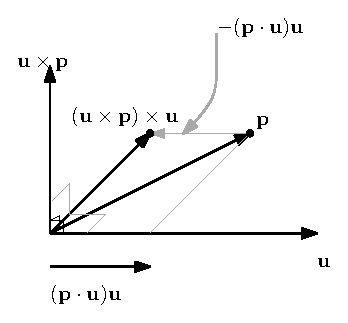
\includegraphics[width=3cm]{Math_quaternion/uxpxu.eps}
\end{figure}

\begin{itemize}
\item $\mathbf u \times \mathbf p \times \mathbf u$는 $\mathbf p - (\mathbf u \cdot \mathbf p) \mathbf u$
\item $\mathbf u \times \mathbf p \times \mathbf u$는 $\mathbf u$와 $\mathbf u \times \mathbf p$에 동시에 수직인 직교축
\item 길이는 $\mathbf p$와 $\mathbf u$의 내적을 통해 알 수 있고, 이를 $\mathbf u$ 축의 음의 방향으로 떨어트리면 됨
\item $\mathbf u \times \mathbf p \times \mathbf u = \mathbf p - (\mathbf p \cdot \mathbf u) \mathbf u$
\end{itemize}

\begin{eqnarray}\nonumber
\hat q \hat p \hat q^* =  ( 0, (\cos^2 \theta - \sin^2 \theta ) \mathbf p + 2 \sin \theta \cos \theta \mathbf u \times \mathbf p + (2 \sin^2 \theta \mathbf u \cdot \mathbf p) \mathbf u ) \nonumber
\end{eqnarray}

\end{frame}
%%%%%%%%%%%%%%%%%%%%%%%%%%%%%%%%%%%%%%%%%%%%%%%%%%%%%%%%%

%%%%%%%%%%%%%%%%%%%%%%%%%%%%%%%%%%%%%%%%%%%%%%%%%%%%%%%%%
\begin{frame}[fragile]{사원수와 회전: 일반적 경우 4/7}

\begin{eqnarray}\nonumber
\cos 2 \theta  & = & \cos^2 \theta - \sin^2 \theta \\ \nonumber
\sin 2 \theta & = & 2 \sin \theta \cos \theta \nonumber
\end{eqnarray}

이 항등식을 적용하면 다음을 얻을 수 있다.

$$\hat q \hat p \hat q^* =  ( 0, (\cos 2\theta \mathbf p + \sin 2 \theta (\mathbf u \times \mathbf p) + (2 \sin^2 \theta \mathbf u \cdot \mathbf p) \mathbf u)$$

\begin{itemize}
\item $1=\cos^2 \theta + \sin^2 \theta$이므로 $\sin^2 \theta = 1 - \cos^2 \theta$
\item $2\sin^2 \theta$는 $\sin^2 \theta + \sin^2 \theta = \sin^2 \theta + 1 - \cos^2 \theta$
\item $1 - (\cos^2 \theta - \sin^2 \theta)$이므로 다음 성립
	\begin{itemize}
	\item $2 \sin^2 \theta = 1 - \cos 2 \theta$
	\end{itemize}
\end{itemize}

$$\hat q \hat p \hat q^* =  ( 0, (\cos 2\theta \mathbf p + \sin 2 \theta (\mathbf u \times \mathbf p) + ((1-\cos 2 \theta) \mathbf u \cdot \mathbf p) \mathbf u)$$

\end{frame}
%%%%%%%%%%%%%%%%%%%%%%%%%%%%%%%%%%%%%%%%%%%%%%%%%%%%%%%%%

%%%%%%%%%%%%%%%%%%%%%%%%%%%%%%%%%%%%%%%%%%%%%%%%%%%%%%%%%
\begin{frame}[fragile]{사원수와 회전: 일반적 경우 5/7}

\begin{figure}
    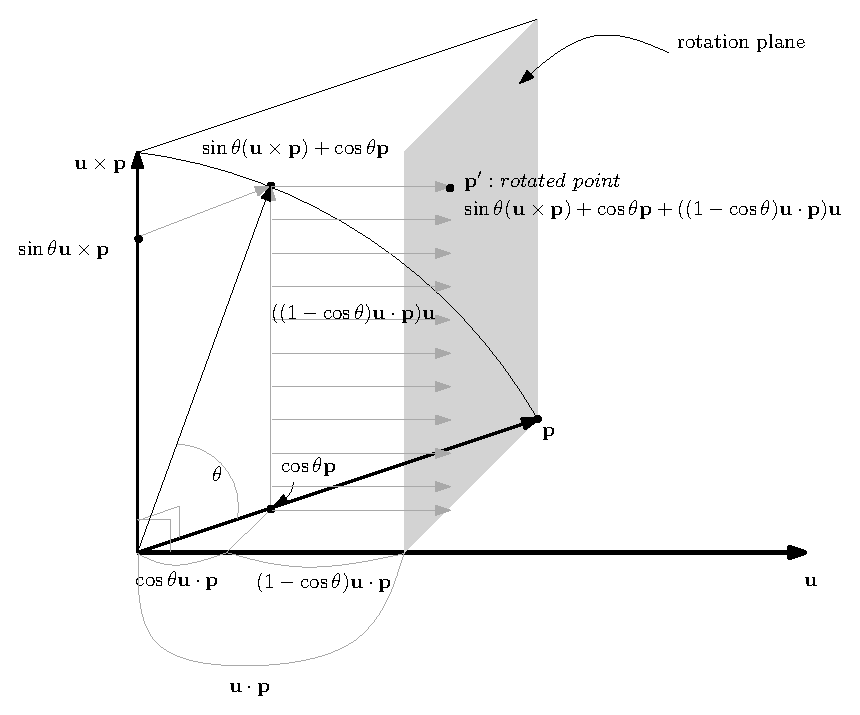
\includegraphics[width=10cm]{Math_quaternion/quaternionRotation.eps}
\end{figure}

\end{frame}
%%%%%%%%%%%%%%%%%%%%%%%%%%%%%%%%%%%%%%%%%%%%%%%%%%%%%%%%%

%%%%%%%%%%%%%%%%%%%%%%%%%%%%%%%%%%%%%%%%%%%%%%%%%%%%%%%%%
\begin{frame}[fragile]{사원수와 회전: 일반적 경우 6/7}

\begin{itemize}
\item 점 $\mathbf p$가 축 $\mathbf u$를 기준으로 회전
\item 회전 과정에 지나는 곡선이 놓인 회색 평면 = 회전 평면
\item $\mathbf p$와 $\mathbf u \times \mathbf p$가 만드는 평면의 원점을 기준을 $\theta$ 만큼 회전하여 얻는 점
	\begin{itemize}
	\item 이 점은 $\mathbf p$ 축으로의 길이는 $|\mathbf p| \cos \theta$
	\item 이 점의 $\mathbf u \times \mathbf p$축 방향으로의 길이는 $|\mathbf p| \sin \theta $
	\item $\sin \theta (\mathbf u \times \mathbf p) + \cos \theta \mathbf p$
	\item 이 점을 회전 평면 위로 옮기면 원하는 좌표
	\end{itemize}
\item 회전 평면으로 옮기는 데에 필요한 길이는 $(1 - \cos \theta) \mathbf u \cdot \mathbf p$
\item 이 길이만큼 $\mathbf u$ 축으로 옮겨 놓는 벡터는 $((1-\cos \theta ) \mathbf u \cdot \mathbf p ) \mathbf u$
\end{itemize}

회전의 결과 좌표는 

$$\mathbf p' = \sin \theta (\mathbf u \times \mathbf p) + \cos \theta \mathbf p +((1-\cos \theta ) \mathbf u \cdot \mathbf p ) \mathbf u$$

\end{frame}
%%%%%%%%%%%%%%%%%%%%%%%%%%%%%%%%%%%%%%%%%%%%%%%%%%%%%%%%%

%%%%%%%%%%%%%%%%%%%%%%%%%%%%%%%%%%%%%%%%%%%%%%%%%%%%%%%%%
\begin{frame}[fragile]{사원수와 회전: 일반적 경우 7/7}


$$\mathbf p' = \sin \theta (\mathbf u \times \mathbf p) + \cos \theta \mathbf p +((1-\cos \theta ) \mathbf u \cdot \mathbf p ) \mathbf u$$

\begin{block}{어떤 점 $\mathbf p$를 $\mathbf u$ 축을 중심으로 $\theta$ 만큼 회전하여 $\mathbf p'$를 얻고 싶을 때}
	\begin{itemize}
	\item $\hat p = (0, \mathbf p)$
	\item $\hat q = (\cos \frac{\theta}{2}, \sin \frac{\theta}{2} \mathbf u)$
	\item $\hat p' = (0, \mathbf p') = \hat q \hat p \hat q^* $
	\end{itemize}
\end{block}

\end{frame}
%%%%%%%%%%%%%%%%%%%%%%%%%%%%%%%%%%%%%%%%%%%%%%%%%%%%%%%%%

%%%%%%%%%%%%%%%%%%%%%%%%%%%%%%%%%%%%%%%%%%%%%%%%%%%%%%%%%
\begin{frame}[fragile]{사원수의 보간}

\begin{itemize}
\item 사원수가 회전을 의미한다면, 그래픽스에서 두 사원수를 보간하는 일은 빈번
\item 보간: $t=0$에서 ${\hat q}_0$이고, $t=1$에서 ${\hat q}_1$인 사원수 ${\hat q}_t$ 구하기
\item 사원수는 행렬에 비해 보간이 쉽다는 장점
\end{itemize}

\begin{figure}
    \includegraphics[width=5cm]{Math_quaternion/QSlerp.png}
\end{figure}

$${\hat q}_0 = (s_0 , u_0, v_0, w_0 )$$
$${\hat q}_1 = (s_1 , u_1, v_1, w_1 )$$

\end{frame}
%%%%%%%%%%%%%%%%%%%%%%%%%%%%%%%%%%%%%%%%%%%%%%%%%%%%%%%%%

%%%%%%%%%%%%%%%%%%%%%%%%%%%%%%%%%%%%%%%%%%%%%%%%%%%%%%%%%
\begin{frame}[fragile]{사원수의 보간: 단순한 선형보간}

\begin{itemize}
\item 간단한 선형보간
	\begin{itemize}
	\item ${\hat q}_t = ( t s_1 + (1-t) s_0 , t u_1 + (1-t) u_0 , t v_1 + (1-t) v_0 , t w_1 + (1-t) w_0)$
	\item 즉, ${\hat q}_t = t {\hat q}_1 + (1-t) {\hat q}_0 $
	\end{itemize}
\item 매우 간단하고 빠르다는 장점
\item 보간이 적용되는 동안 사원수의 길이가 길이가 변하는 단점
\end{itemize}

\begin{figure}
    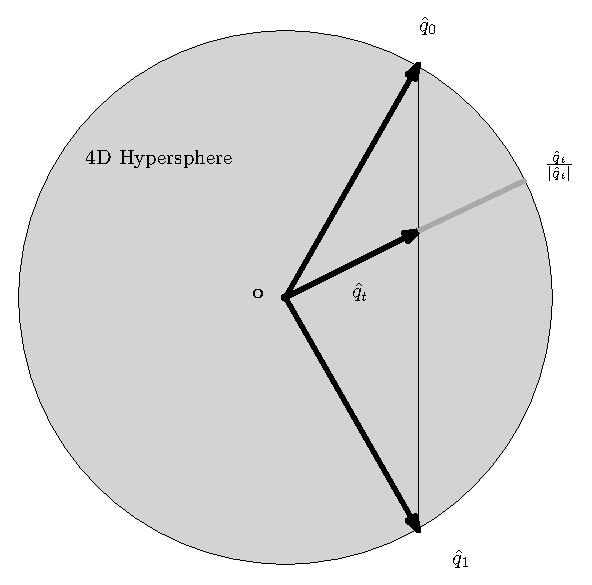
\includegraphics[width=5cm]{Math_quaternion/quaternionLerp.eps}
\end{figure}

\end{frame}
%%%%%%%%%%%%%%%%%%%%%%%%%%%%%%%%%%%%%%%%%%%%%%%%%%%%%%%%%

%%%%%%%%%%%%%%%%%%%%%%%%%%%%%%%%%%%%%%%%%%%%%%%%%%%%%%%%%
\begin{frame}[fragile]{사원수의 보간: 간단한 개선 방법}

\begin{itemize}
\item 사원수가 항상 초구면의 표면에 있도록 그 길이를 조정
\item ${\hat q}_t / | {\hat q}_t |$로 정규화
\item 길이는 유지되지만 회전속도는 일정하지 않음
	\begin{itemize}
	\item 극단적인 상황: ${\hat q}_0$와 ${\hat q}_1$이 서로 반대 방향
		\begin{itemize}
		\item 선형 보간하여 얻는 사원수는 $t=0.5$가 될 때까지는 초기의 회전각
		\item $t=0.5$ 시점을 지나면 바로 다음 회전각으로 전환
		\end{itemize}
	\end{itemize}
\end{itemize}

사원수의 단순한 선형보간으로 얻어지는 각도의 변화와 각속도의 변화
\begin{figure}
  	\begin{tabular}{cc}
	 \multicolumn{2}{c}{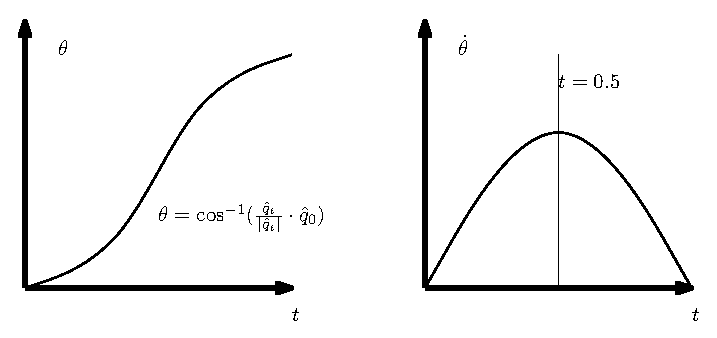
\includegraphics[width=9cm]{Math_quaternion/quaternionLerpAngle.eps}} \\
	(a) 각도의 변화 & (b) 각속도의 변화 \\
	\end{tabular}
\end{figure}

\end{frame}
%%%%%%%%%%%%%%%%%%%%%%%%%%%%%%%%%%%%%%%%%%%%%%%%%%%%%%%%%

%%%%%%%%%%%%%%%%%%%%%%%%%%%%%%%%%%%%%%%%%%%%%%%%%%%%%%%%%
\begin{frame}[fragile]{사원수의 보간: 구면보간(球面補間) 혹은 Slerp}

\begin{itemize}
\item 사원수의 보간은 각도 $\theta$가 선형으로 보간되어야 함
\end{itemize}

구면 보간을 통해 얻어야 하는 사원수 보간의 각도의 변화와 각속도의 변화

\begin{figure}
  	\includegraphics[width=9cm]{Math_quaternion/quaternionSlerpAngle.eps}
\end{figure}

\end{frame}
%%%%%%%%%%%%%%%%%%%%%%%%%%%%%%%%%%%%%%%%%%%%%%%%%%%%%%%%%

%%%%%%%%%%%%%%%%%%%%%%%%%%%%%%%%%%%%%%%%%%%%%%%%%%%%%%%%%
\begin{frame}[fragile]{구면보간(球面補間): 등각속도 구면보간의 개념}

\begin{itemize}
\item 구면보간
	\begin{itemize}
	\item 시작과 끝 회전을 표현하는 사원수 $\hat q_0$와 $\hat q_1$에 적절한 가중치 $a(t)$와 $b(t)$ 적용
	\item 가중치가 적용된 두 사원수를 합성
	\item 현재 시간 $t$에 제한조건을 만족하는 $a(t)$와 $b(t)$를 찾는 작업
	\end{itemize}
\end{itemize}

\begin{figure}
	\includegraphics[width=8cm]{Math_quaternion/quaternionSlerp.eps}
\end{figure}

\end{frame}
%%%%%%%%%%%%%%%%%%%%%%%%%%%%%%%%%%%%%%%%%%%%%%%%%%%%%%%%%

%%%%%%%%%%%%%%%%%%%%%%%%%%%%%%%%%%%%%%%%%%%%%%%%%%%%%%%%%
\begin{frame}[fragile]{구면보간(球面補間): $a(t)$ 구하기}

\begin{itemize}
\item $\hat q_0$에서 $\hat q_1$까지의 회전각 전체가 $\theta_d$
\item 시간 $t$에서 보간된 사원수 $\hat q_t$와 $\hat q_0$가 이루는 각이 $\theta_t$
\item $\theta_d$에서 $\theta_t$를 뺀 각도를 $\theta_{1-t}$
\item $a(t)$와 $|\hat q_0 |$의 비(比)는 결국 $|\hat q_t| \sin \theta_{1-t}$와 $|\hat q_0| \sin \theta_d$의 비
\item $a(t) = \frac{\sin \theta_{1-t}}{\sin \theta_d} $
\end{itemize}

\begin{figure}
	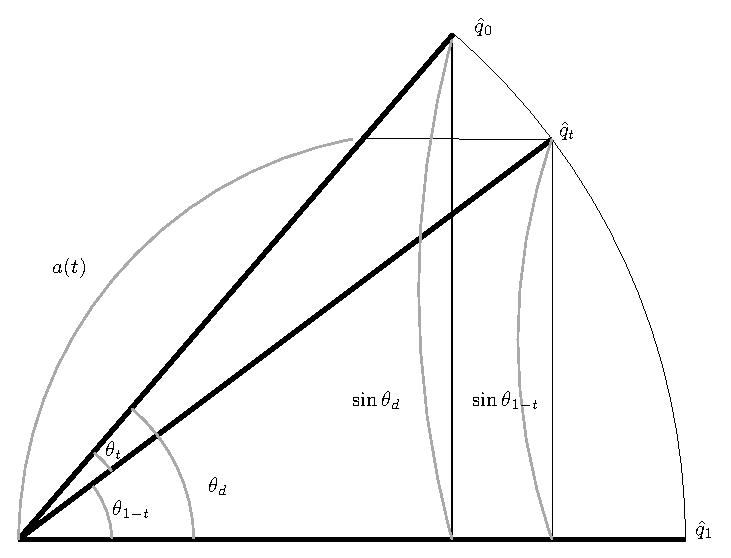
\includegraphics[width=6cm]{Math_quaternion/quaternionSlerpA.eps}
\end{figure}

\end{frame}
%%%%%%%%%%%%%%%%%%%%%%%%%%%%%%%%%%%%%%%%%%%%%%%%%%%%%%%%%

%%%%%%%%%%%%%%%%%%%%%%%%%%%%%%%%%%%%%%%%%%%%%%%%%%%%%%%%%
\begin{frame}[fragile]{구면보간(球面補間): $b(t)$ 구하기}

\begin{itemize}
\item $b(t)$와 $|\hat q_1$의 비는 $|\hat q_t | \sin \theta_t$의 값과 $|\hat q_1 | \sin \theta_d$가 이루는 비
\item $b(t) = \frac{\sin \theta_{t}}{\sin \theta_d} $
\end{itemize}

\begin{figure}
	\includegraphics[width=8cm]{Math_quaternion/quaternionSlerpB.eps}
\end{figure}


\end{frame}
%%%%%%%%%%%%%%%%%%%%%%%%%%%%%%%%%%%%%%%%%%%%%%%%%%%%%%%%%

%%%%%%%%%%%%%%%%%%%%%%%%%%%%%%%%%%%%%%%%%%%%%%%%%%%%%%%%%
\begin{frame}[fragile]{구면보간(球面補間) 계산법}

\begin{itemize}
\item $a(t)$와 $b(t)$를 구하고 나면, 보간된 사원수 $\hat q_t$
\item $\hat q_t = a(t) \hat q_0 + b(t) \hat q_1$
\end{itemize}

\begin{itemize}
\item 사원수가 동일한 각속도로 부드럽게 보간된다. 이러한 보간 방법은 구면보간
\item ``slerp"이라는 이름으로 종종 부름
\item 이때 사원수의 크기는 언제나 1
\end{itemize}

\begin{eqnarray} \nonumber
\theta_d & = & \cos^{-1} (\hat q_0 \cdot \hat q_1) \\ \nonumber
s & = & \sin \theta_d = \sqrt{1 - (\hat q_0 \cdot \hat q_1)^2} \\ \nonumber
\hat q_t & = & \frac{\sin \theta_{1-t}}{s} \hat q_0+ \frac{\sin \theta_t}{s} \hat q_1 \nonumber
\end{eqnarray}


\end{frame}
%%%%%%%%%%%%%%%%%%%%%%%%%%%%%%%%%%%%%%%%%%%%%%%%%%%%%%%%%













